\section{Discussion}
%talk about fluorescence maybe
%talk about the next steps, what's to do: check the abundances or check with models. Cite some articles(check the word document). See how many photons would be expected. 
% would be cool to put limits on processes: charge-exchange, fluorescence of heavy elements etc...

    \begin{figure}[H]
        \centering
        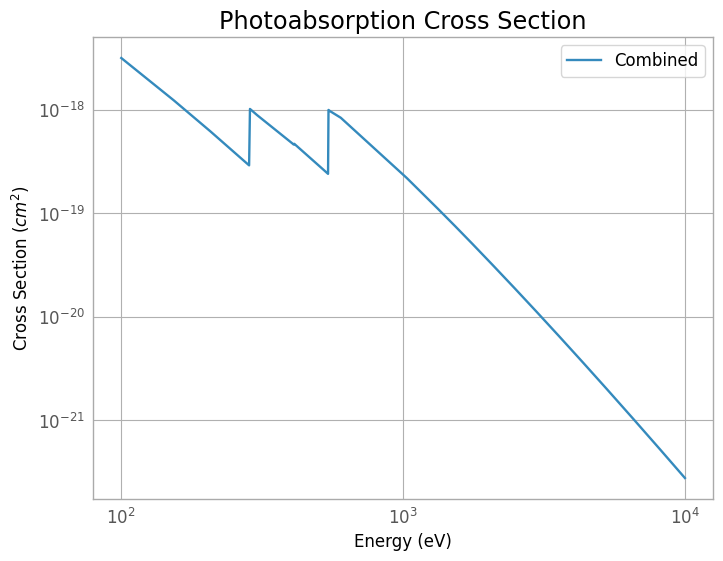
\includegraphics[width = 8cm]{report/Figures/discussion/crosssection.png}
        \caption{Cross-section of Venus' atmosphere using in the range using the \href{https://xraypy.github.io/XrayDB/}{\texttt{Xraydb.sqlite}} database.}
        \label{cross_sec}
    \end{figure}
    